\newpage
\subsection{Morphologischer Kasten}
Die für uns wichtigsten Einflussfaktoren verwenden wir für den morphologischen Kasten (Abb. \ref{fig:MorphologischerKasten}), um unsere Geschäftsidee zu konkretisieren.

\begin{figure}[H]
\centering
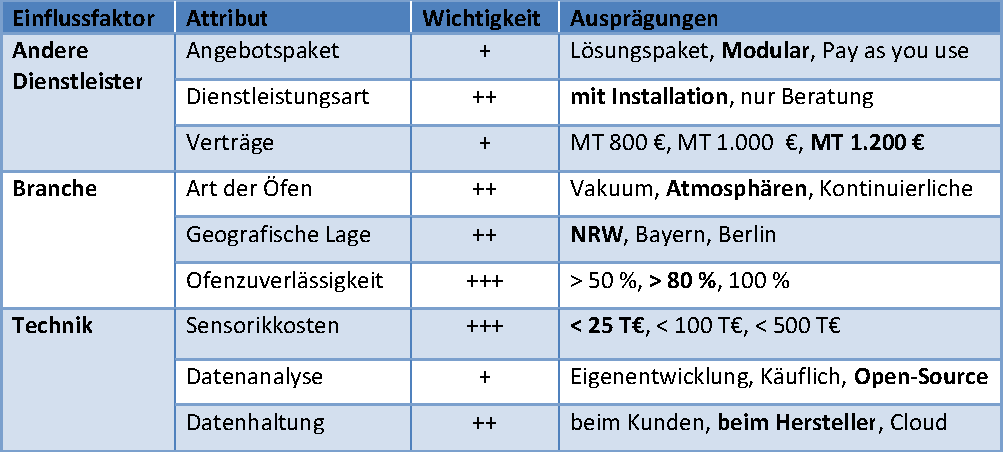
\includegraphics[width=0.9\linewidth]{Bilder/MorphologischerKasten}
\caption{Unser morphologischer Kasten}
\label{fig:MorphologischerKasten}
\end{figure}

Wir möchten als IT-Dienstleister im Bereich Predictive Maintenance mit einem Hersteller von Atmosphärenöfen zusammenarbeiten. Dabei konzentrieren wir uns auf Hersteller im Raum NRW, deren Öfen eine Zuverlässigkeit von mehr als 80 Prozent aufweisen. Für die Messung der Daten verwenden wir Sensorik deren Kosten unterhalb von 25.000 Euro liegen. Zur Analyse werden die Daten beim Ofenhersteller gespeichert und im Wesentlichen mit Hilfe von Open-Source-Lösungen ausgewertet. Unsere Angebotspakete sind modular aufgebaut, so dass aus unserem Dienstleistungsportfolio unterschiedliche Ausbaustufen in Anspruch genommen werden können. Neben der reinen Beratungsleistung bieten wir zusätzlich auch die Möglichkeit diese zu installieren. Für unsere Dienstleistung berechnen wir einen Tagessatz von 1.2000 Euro.
